%!TEX TS-program = xelatex
\documentclass[11pt]{article}

\usepackage[english]{babel}

\usepackage{amsmath}
\usepackage[T1]{fontenc}

\usepackage{geometry}
\usepackage{setspace}

\usepackage[hang,flushmargin]{footmisc}

\setlength{\parindent}{0pt}
\setlength{\parskip}{6pt plus 2pt minus 1pt}\providecommand{\tightlist}{%
  \setlength{\itemsep}{0pt}\setlength{\parskip}{0pt}}

\makeatletter
\newcounter{tableno}
\newenvironment{tablenos:no-prefix-table-caption}{
  \caption@ifcompatibility{}{
    \let\oldthetable\thetable
    \let\oldtheHtable\theHtable
    \renewcommand{\thetable}{tableno:\thetableno}
    \renewcommand{\theHtable}{tableno:\thetableno}
    \stepcounter{tableno}
    \captionsetup{labelformat=empty}
  }
}{
  \caption@ifcompatibility{}{
    \captionsetup{labelformat=default}
    \let\thetable\oldthetable
    \let\theHtable\oldtheHtable
    \addtocounter{table}{-1}
  }
}
\makeatother

\usepackage{array}
\newcommand{\PreserveBackslash}[1]{\let\temp=\\#1\let\\=\temp}
\let\PBS=\PreserveBackslash

\usepackage[breaklinks=true]{hyperref}
\hypersetup{colorlinks,%
citecolor=blue,%
filecolor=blue,%
linkcolor=blue,%
urlcolor=blue}
\usepackage{url}

\usepackage{caption}
\setcounter{secnumdepth}{0}
\usepackage{cleveref}

\usepackage{graphicx}
\makeatletter
\def\maxwidth{\ifdim\Gin@nat@width>\linewidth\linewidth
\else\Gin@nat@width\fi}
\makeatother
\let\Oldincludegraphics\includegraphics
\renewcommand{\includegraphics}[1]{\Oldincludegraphics[width=\maxwidth]{#1}}

\usepackage{longtable}
\usepackage{booktabs}

\usepackage{color}
\usepackage{fancyvrb}
\newcommand{\VerbBar}{|}
\newcommand{\VERB}{\Verb[commandchars=\\\{\}]}
\DefineVerbatimEnvironment{Highlighting}{Verbatim}{commandchars=\\\{\}}
% Add ',fontsize=\small' for more characters per line
\usepackage{framed}
\definecolor{shadecolor}{RGB}{248,248,248}
\newenvironment{Shaded}{\begin{snugshade}}{\end{snugshade}}
\newcommand{\KeywordTok}[1]{\textcolor[rgb]{0.13,0.29,0.53}{\textbf{#1}}}
\newcommand{\DataTypeTok}[1]{\textcolor[rgb]{0.13,0.29,0.53}{#1}}
\newcommand{\DecValTok}[1]{\textcolor[rgb]{0.00,0.00,0.81}{#1}}
\newcommand{\BaseNTok}[1]{\textcolor[rgb]{0.00,0.00,0.81}{#1}}
\newcommand{\FloatTok}[1]{\textcolor[rgb]{0.00,0.00,0.81}{#1}}
\newcommand{\ConstantTok}[1]{\textcolor[rgb]{0.00,0.00,0.00}{#1}}
\newcommand{\CharTok}[1]{\textcolor[rgb]{0.31,0.60,0.02}{#1}}
\newcommand{\SpecialCharTok}[1]{\textcolor[rgb]{0.00,0.00,0.00}{#1}}
\newcommand{\StringTok}[1]{\textcolor[rgb]{0.31,0.60,0.02}{#1}}
\newcommand{\VerbatimStringTok}[1]{\textcolor[rgb]{0.31,0.60,0.02}{#1}}
\newcommand{\SpecialStringTok}[1]{\textcolor[rgb]{0.31,0.60,0.02}{#1}}
\newcommand{\ImportTok}[1]{#1}
\newcommand{\CommentTok}[1]{\textcolor[rgb]{0.56,0.35,0.01}{\textit{#1}}}
\newcommand{\DocumentationTok}[1]{\textcolor[rgb]{0.56,0.35,0.01}{\textbf{\textit{#1}}}}
\newcommand{\AnnotationTok}[1]{\textcolor[rgb]{0.56,0.35,0.01}{\textbf{\textit{#1}}}}
\newcommand{\CommentVarTok}[1]{\textcolor[rgb]{0.56,0.35,0.01}{\textbf{\textit{#1}}}}
\newcommand{\OtherTok}[1]{\textcolor[rgb]{0.56,0.35,0.01}{#1}}
\newcommand{\FunctionTok}[1]{\textcolor[rgb]{0.00,0.00,0.00}{#1}}
\newcommand{\VariableTok}[1]{\textcolor[rgb]{0.00,0.00,0.00}{#1}}
\newcommand{\ControlFlowTok}[1]{\textcolor[rgb]{0.13,0.29,0.53}{\textbf{#1}}}
\newcommand{\OperatorTok}[1]{\textcolor[rgb]{0.81,0.36,0.00}{\textbf{#1}}}
\newcommand{\BuiltInTok}[1]{#1}
\newcommand{\ExtensionTok}[1]{#1}
\newcommand{\PreprocessorTok}[1]{\textcolor[rgb]{0.56,0.35,0.01}{\textit{#1}}}
\newcommand{\AttributeTok}[1]{\textcolor[rgb]{0.77,0.63,0.00}{#1}}
\newcommand{\RegionMarkerTok}[1]{#1}
\newcommand{\InformationTok}[1]{\textcolor[rgb]{0.56,0.35,0.01}{\textbf{\textit{#1}}}}
\newcommand{\WarningTok}[1]{\textcolor[rgb]{0.56,0.35,0.01}{\textbf{\textit{#1}}}}
\newcommand{\AlertTok}[1]{\textcolor[rgb]{0.94,0.16,0.16}{#1}}
\newcommand{\ErrorTok}[1]{\textcolor[rgb]{0.64,0.00,0.00}{\textbf{#1}}}
\newcommand{\NormalTok}[1]{#1}

\newlength{\cslhangindent}
\setlength{\cslhangindent}{1.5em}
\newlength{\csllabelwidth}
\setlength{\csllabelwidth}{3em}
\newenvironment{CSLReferences}[3] % #1 hanging-ident, #2 entry spacing
 {% don't indent paragraphs
  \setlength{\parindent}{0pt}
  % turn on hanging indent if param 1 is 1
  \ifodd #1 \everypar{\setlength{\hangindent}{\cslhangindent}}\ignorespaces\fi
  % set entry spacing
  \ifnum #2 > 0
  \setlength{\parskip}{#2\baselineskip}
  \fi
 }%
 {}
\usepackage{calc} % for \widthof, \maxof
\newcommand{\CSLBlock}[1]{#1\hfill\break}
\newcommand{\CSLLeftMargin}[1]{\parbox[t]{\maxof{\widthof{#1}}{\csllabelwidth}}{#1}}
\newcommand{\CSLRightInline}[1]{\parbox[t]{\linewidth}{#1}}
\newcommand{\CSLIndent}[1]{\hspace{\cslhangindent}#1}
\geometry{verbose,letterpaper,tmargin=2.2cm,bmargin=2.2cm,lmargin=2.2cm,rmargin=5cm}

\pagestyle{plain}

\begin{document}

{\LARGE\bfseries Preprint template}

\vskip 2em

{\small
Timothée\,Poisot\,\textsuperscript{1,2,*}, Peregrin\,Took\,\textsuperscript{3,4}, Merriadoc\,Brandybuck\,\textsuperscript{5,4}
\vskip 1em
\textsuperscript{1}\,Université de Montréal; \textsuperscript{2}\,Québec
Centre for Biodiversity Sciences; \textsuperscript{3}\,Inn of the
Prancing Pony; \textsuperscript{4}\,Fellowship of the
Ring; \textsuperscript{5}\,Green Dragon Inn\\
\textsuperscript{*}\,\,\texttt{timothee.poisot@umontreal.ca}
}

\vskip 2em

\textbf{Abstract:}\,This template is used by the Poisot lab at
Université de Montréal to write manuscripts using github. It uses github
actions as a way to generate a website that can be annotated using
hypothes.is, a PDF document for copy-editing and submission to journals,
and a PDF document for submission to preprint servers. At every push on
the master branch, the whole series of documents will get built.

\vskip 2em

This template uses recent versions of \texttt{pandoc} and
\texttt{pandoc-crossref} to faciltate the referencing of equations,
figures, and tables within the text. For example, the following equation

\begin{equation}\protect\hypertarget{eq:eq1}{}{J'(p) = \frac{1}{\text{log}(S)}\times\left(-\sum p \times \text{log}(p)\right)}\label{eq:eq1}\end{equation}

is produced using

\begin{Shaded}
\begin{Highlighting}[]
\SpecialStringTok{$$J\textquotesingle{}(p) = }\SpecialCharTok{\textbackslash{}frac}\SpecialStringTok{\{1\}\{}\SpecialCharTok{\textbackslash{}text}\NormalTok{\{log\}}\SpecialStringTok{(S)\}}\SpecialCharTok{\textbackslash{}times\textbackslash{}left}\SpecialStringTok{({-}}\SpecialCharTok{\textbackslash{}sum}\SpecialStringTok{ p }\SpecialCharTok{\textbackslash{}times}\SpecialStringTok{ }\SpecialCharTok{\textbackslash{}text}\NormalTok{\{log\}}\SpecialStringTok{(p)}\SpecialCharTok{\textbackslash{}right}\SpecialStringTok{)$$}\NormalTok{ \{\#eq:eq1\}}
\end{Highlighting}
\end{Shaded}

and can be referenced using \texttt{@eq:eq1}, which will result in
eq.~\ref{eq:eq1}.

All documents will be deployed to \texttt{gh-pages} \emph{only} on push
events from the \texttt{master} All of the artifacts will be built when
doing pull requests, so you can check that merging a branch is
\emph{not} going to cause the compilation of the documents to fail.

\hypertarget{using-references}{%
\section{Using references}\label{using-references}}

The references are managed by the \texttt{citeproc} filter for
\texttt{pandoc}. Note that we \emph{do not} use
\texttt{pandoc-citeproc}, which was an external moduler for older
\texttt{pandoc} versions. References \emph{have to} be stored in a
\texttt{references.bib} file. We use
\href{https://www.zotero.org/}{Zotero} for references management, and
for the lab's manuscripts, we work from folders in a shared library
(with a folder for every manuscript).

We use the \href{https://retorque.re/zotero-better-bibtex/}{Better
BibTeX} plugin for citation key generations, and auto-export of the
shared library to the \texttt{references.bib} file. We use a citation
key format meant to convey information on the author, date, year, and
title. It must be set in the Better BibTeX preferences as

\begin{verbatim}
[auth:fold][year][title:fold:nopunctordash:skipwords:lower:select=1,1:substring=1,3:capitalize][title:fold:nopunctordash:skipwords:lower:select=2,2:substring=1,3:capitalize]
\end{verbatim}

The citations are done using normal markdown, where
\texttt{@Elton1927AniEco} produces Elton (1927), and
\texttt{{[}@Camerano1880EquViv{]}} produces (Camerano 1880).

\hypertarget{tables}{%
\section{Tables}\label{tables}}

Tables are supported in their normal markdown way:

\begin{longtable}[]{@{}lrc@{}}
\toprule
Column 1 & Column 2 & Column 3\tabularnewline
\midrule
\endhead
c1 & c2 & c3\tabularnewline
c2 & c3 & c4\tabularnewline
c5 & c6 & c7\tabularnewline
\bottomrule
\end{longtable}

\hypertarget{figures}{%
\section{Figures}\label{figures}}

Figures can have a legend -- all figures \emph{must} be in the
\texttt{figures/} folder of the project:

\begin{verbatim}
![This is the legend of the figure](figures/biomes.png){#fig:biomes}
\end{verbatim}

\begin{figure}
\hypertarget{fig:biomes}{%
\centering
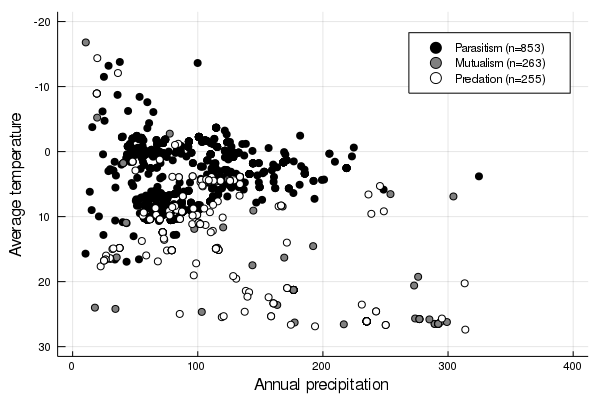
\includegraphics{figures/biomes.png}
\caption{This is the legend of the figure}\label{fig:biomes}
}
\end{figure}

We can now use \texttt{@fig:biomes} to refer to fig.~\ref{fig:biomes}.

\hypertarget{references}{%
\section*{References}\label{references}}
\addcontentsline{toc}{section}{References}

\hypertarget{refs}{}
\begin{CSLReferences}{1}{0}
\leavevmode\hypertarget{ref-Camerano1880EquViv}{}%
Camerano, Lorenzo. 1880. {``Dell'equilibrio Dei Viventi Merce La
Reciproca Distruzione.''} \emph{Atti Della R. Accad. Delle Sci. Torino}
15: 393--414.

\leavevmode\hypertarget{ref-Elton1927AniEco}{}%
Elton, Charles S. 1927. \emph{Animal Ecology}. University of Chicago
Press.

\end{CSLReferences}

\end{document}
